\chapter{Global fitting algorithm details \label{chap:Fit}}
This Appendix is devoted to the method used to extract the fitting parameters from the Raman line scans discussed in Chapter \ref{chap:fri}.
Throughout, fitting parameters refers to the non-linear parameters of interest, namely the dimensionless friction, $F$, the Gru\"uneisen parameter, $\gamma$, and the shear deformation potential, $\beta$.
The determination of these values is complicated; there is no out of the box technique which can be blindly applied.
Additionally it is computationally expensive.
The fits including all three fitting parameters took two days to run on 7 processors.
Accordingly, this Appendix will endeavor to give enough detail to easily reproduce the fitting algorithm while providing tricks to maximize efficiency in Wolfram Mathematica 8.0 along the way.

Since the functional dependencies of the fitted parameters is very complicated and non-linear, an out of the box fitting algorithm can not be applied.
Instead, a brute force algorithm is used to determine the fitting parameters.
A range of fitting parameters sets, ($F$,$\gamma$,$\beta$), are iterated through and for each set the global reduced $\chi^2$, 
\begin{equation*}
	\tilde{\chi}^2=\frac{1}{D.O.F.} \sum_i \left( \frac{model_i-data_i}{\sigma_i} \right)^2 \ ,
\end{equation*}
is calculated as a goodness of fit metric.
Here, $D.O.F.$ is the degrees of freedom in the fit equal to the number of data points fit minus the number of parameters fit to the data, $model_i-data_i$ is the difference between the modeled and measured values at point $i$, and $\sigma_i$ is the measured uncertainty in $data_i$.
Most importantly, $i$ includes the data points from \emph{all} of the spectra in the line scan.
Instead of fitting each spectra individually, the full line scan is taken into account for a global determination of the fitting parameters.
The best fit value is then found by looking for the fitting parameters which yield the smallest $\tilde{\chi}^2$.

The algorithm used to find the best fit is detailed in the flowchart in Figure \ref{fig:Fit:Flow}.
Broadly speaking, the algorithm works by looping across a range of fitting parameters and checking how accurately the fitting parameters represent the global line scan spectra.
Individual steps are described in the proceeding.
Steps with red outlines in the flowchart will be described in the most detail as they are the most difficult.

\begin{figure}
	\begin{center}
	\newcommand{\fctw}{1.5in}
\newcommand{\fcmh}{6mm}
\resizebox{!}{7.5in}{
\begin{tikzpicture}[node distance=5 mm,
	terminal/.style={rectangle, rounded corners=3mm, 
				minimum height=\fcmh, text width=\fctw, text centered,
				very thick, draw=green!50!black, fill=black!5},
	process/.style={rectangle, rounded corners=1.5mm,
				minimum height=\fcmh, text width=\fctw, text centered,
				very thick, draw=blue!50!black, fill=black!5},
	pprocess/.style={rectangle,rounded corners=1.5mm,
				minimum height=\fcmh, text width=\fctw, text centered,,
				ultra thick, draw=red!50!black, fill=black!5},
	decision/.style={diamond, aspect=2,
				minimum height=\fcmh, text width=\fctw, text badly centered, inner sep=0,
				very thick, draw=black, fill=black!5},
	data/.style={trapezium, trapezium left angle=70, trapezium right angle=-70,
				minimum height=\fcmh, text width=\fctw, text centered, 
				very thick, draw=orange!50, fill=black!5},
	line/.style={draw,thick,-latex'}
	]

	\node (load)	[terminal]
		{Load spectra, known parameters};
	\node (setFGB)	[process,below=of load]
		{First $F$, $\gamma$, $\beta$};
	\node (strain)	[process,below=of setFGB]
		{Hypothesize strains};
	\node (first)	[process,below=of strain]
		{First spectra};
	\node (getrho)	[pprocess,below=of first]
		{Determine $\rho$};
	\node (nextr)	[process,left=of getrho]
		{Next spectra};
	\node (isin)	[decision,below=of getrho]
		{Fit $\rho$?};
	\node (rdom)	[process,below=of isin]
		{Restrict fit domain};
	\node (pspec)	[pprocess,below=of rdom]
		{Predict spectral shape};
	\node (linc)	[pprocess,below=of pspec]
		{Fit linear coefficients};
	\node (chi2)	[process,below=of linc]
		{Add $\chi^2$ to global $\chi^2$};
	\node (rleft)	[decision,below=of chi2]
		{Last spectra?};
	\node (Fleft)	[decision,below=of rleft]
		{Last fitting values?};
	\node (nextF)	[process,right=of getrho]
		{Next $F$, $\gamma$, $\beta$};
	\node (end)		[terminal,below=of Fleft]
		{Select best $\tilde{\chi}^2$ and estimate errors};

	\draw[line] (load)	--	(setFGB);
	\draw[line] (setFGB)--	(strain);
	\draw[line] (strain)--	(first);
	\draw[line]	(first)	--	(getrho);
	\draw[line] (getrho)--	(isin);
	\draw[line]	(isin) 	--	node[anchor=west]{yes}	(rdom);
	\draw[line]	(isin)	-|	node[near start,anchor=south]{no}	(nextr);
	\draw[line]	(nextr) |-	($(first.south) + (0,-2.5mm)$);
	\draw[line]	(rdom)	--	(pspec);
	\draw[line] (pspec) --	(linc);
	\draw[line]	(linc)	--	(chi2);
	\draw[line] (chi2)	--	(rleft);
	\draw[line]	(rleft)	--	node[anchor=west]{yes} (Fleft);
	\draw[line] (Fleft) -- 	node[anchor=west]{yes} (end);
	\draw[line]	(rleft) -|	node[near start,anchor=south]{no}	(nextr);
	\draw[line]	(Fleft) -|	node[near start,anchor=south]{no}	(nextF);
	\draw[line]	(nextF)	|-	($(setFGB.south) + (0,-2.5mm)$);
\end{tikzpicture}
}
	\end{center}
	\caption[Flow chart of global fitting algorithm]{\label{fig:Fit:Flow}Flow chart of global fitting algorithm to determine $F$, $\gamma$, $\beta$ from line scans over pressurized graphene sealed microchambers.}
\end{figure}

\section*{Load spectra, known parameters}
The first step is to load in the measured spectra and the independently determined parameters.
There are many free parameters in the system, but the majority of them are measured independently.
The applied pressure is measured using a digital pressure gauge and recorded as a function of time.
Often, the pressure regulator will allow the pressure to decrease by several tenths of a PSI during a measurement.
In this case, the average of the pressure over the measurement window is used.
The determination of the pressure trapped inside the microchamber as well as the unstrained G band position for the suspended FLG is detailed in Section \ref{sec:fri:ambient}.
The G band width for the suspended graphene is taken from the center of the atmospheric pressure line scan.
For supported FLG, the width and position of the unstrained G band is taken from the spectra at the largest radial distance measured during a line scan at either 0.17 MPa or atmospheric pressure.
The number of graphene layers is found using Raman spectroscopy \cite{Ferrari2006} and optical contrast \cite{Blake2007,Casiraghi2007a}.
The measurement of the laser spot size is described in Section \ref{sec:fri:Raman}
Microchamber radius is determined from ambient pressure AFM which is analyzed depending on the devices ambient pressure behavior.
For those devices that bulge up, the radius is found by fitting an AFM section cut which spans the microchamber center with the lowest order approximation to the Hencky model: A parabola.
For those devices which stick to the side walls, the radius is measured manually based on the two dimensional topography.
This leaves only the friction, Gr\"{u}neisen parameter, shear deformation potential, signal intensity, and signal background as unknowns.

\section*{First $F$, $\gamma$, $\beta$}
Next, the outer loop is entered which cycles through the sampled fitting parameters.
A balance must be struck when defining the range of fitting parameters to be tested.
Too few fitting parameters increases the chances of missing the global minimum while too many makes the computational load too high.
Supplementing this fitting algorithm with a manual fitting technique can build an intuition for the system while also decreasing the chances the global minimum is not found.
By guessing individual fitting parameters instead of looping through a range of values, the user can observe how the fitting parameters effect the predicted spectra and $\tilde{\chi}^2$.
This intuition gained should assist the user in determining a reasonable range of fitting parameters.

\section*{Hypothesize strains}
Having selected one set of fitting parameters, the guessed dimensionless friction, $F$, is used with the measured dimensionless loading, $q$, to generate a hypothetical strain distribution.
This amounts to solving Equations \ref{eq:fri:BCs} for the parameters which determine the shape of the strain distribution, $b_0$ and $\rho_0$, given the physical parameters $q$ and $F$.
Mathematica's Solve routine can be effectively used for this, giving a result in several seconds when the series solution for the stress of the suspended graphene includes terms up to tenth order in $\rho$.
The single real solution to these equations defines the hypothetical strain distribution.
The next task is to determine how well the measure spectra agree with this strain distribution.

\section*{First spectra}
The second loop cycles through the spectra in the line scan.
Even though the fitting is global in scope, individual spectra must still be isolated to fit linear coefficients.

\section*{Determine $\rho$}
Even though the distance the sample is moved between spectra is set experimentally, the position of the individual spectra relative to the center of the hole is not necessarily fully determined.
This uncertainty could arise due to a slight offset in the beam position relative to the targeted position, from sample drift, or from targeting uncertainty.
This can be best overcome using a retroactive determination of the central spectra which uses single Lorentzian fits to the data.
When the line scan spectra are fit with a single Lorentzian, the position dependence of the center frequency comes to a symmetric minimum as shown in Figure \ref{fig:fri:qualresults}.
This minimum occurs at the center of the microchamber where the strains, and thus the downshifts, are the greatest.
Its position can be accurately determined by fitting a similar symmetric function to the single Lorentzian fits, such as a Gaussian or a parabola.
The dimensionless radius, $\rho=r/R$, which the spectra was taken at can then be calculated from the position of the center of the microchamber, the spacing between spectra, and the radius of the microchamber.

\section*{Fit $\rho$?}
Not every spectra in the line scan is included in the fit.
When fitting the extended Hencky model to the measured spectra, for microchambers with radii larger than $1.5 \ \mu m$ the global $\chi^2$ includes every spectra in the line scan except for those located less than half the beam waist away from the edge of the microchamber.
This is done to avoid including the additional fitting parameters needed to account for the signal mismatch between suspended and supported FLG created by different optical interference conditions.

When fitting the smaller radius microchambers ($R<1.5 \ \mathrm{\mu m}$), the spectra from the suspended graphene are ignored.
Figure \ref{fig:Fit:igouter} shows an example of the resulting best fit.
Even though they were not included in the fit, the spectra predicted by the extended Hencky model matches the major feature of the suspended spectra.
Spectra from the suspended region ($\rho<1$) exhibit a high energy shoulder that is not predicted by the extended Hencky model.
This feature is observed in each of the three measured graphene sealed microchambers with radius less than $1.5 \ \mathrm{\mu m}$ but not for the five larger radius microchambers.
This feature is believed to come from airy rings in the focused laser beam.
These rings of intensity would contribute signal from lower strain regions giving a distinct higher energy signal, and not a broadening.
For larger radius microchambers, the laser spot is smaller relative to the microchamber radius and so it samples a more uniform distribution of strains, making an extra contribution from the airy rings unimportant.
Complications of fitting these features are avoided by only including the spectra from the supported graphene when fitting.  

\begin{figure}
	\begin{center}
	\begin{tikzpicture}[scale=.675]
	%The spectra
	\node at (0,0) {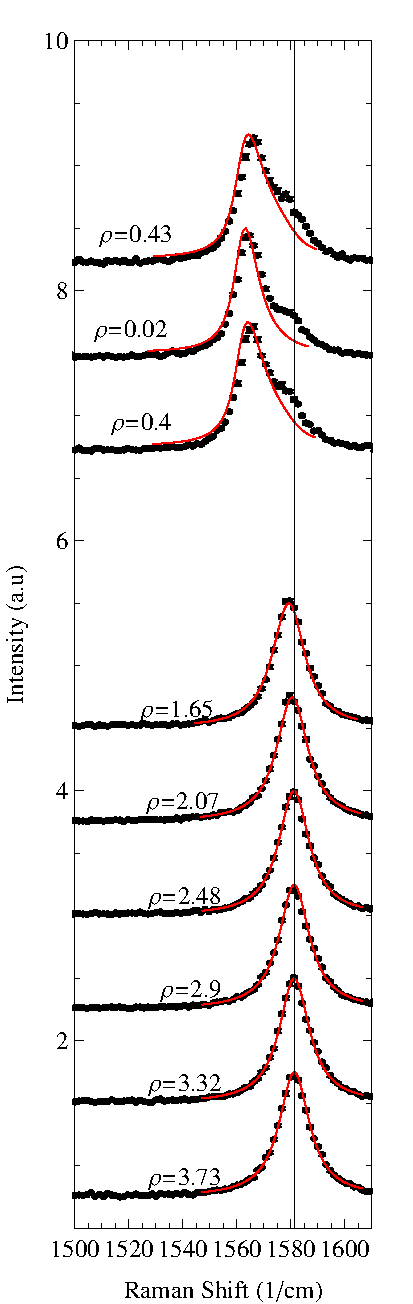
\includegraphics[scale=.675]{Figs_Fit/2012-12-18_Fit_101psi_Spectra_for_paper_sb04-6b.pdf}};
	
	%The picture of the hole
	\newcommand{\arrowlength}{.144*2.4 cm}%.144 is 2.5 um
	\begin{scope}[xshift=-.5 cm,yshift=1.25 cm]
		%For the total scale=1 the .jpg scale is .6
		\node at (0,0) {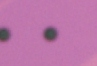
\includegraphics[scale=.30375,angle=-90]{Figs_Fit/SB04-6b.jpg}};%was .225 before I change the scale from .5 to .45
		\draw[->,black,>=stealth] (-.03cm,-\arrowlength-.05 cm-.136 cm) -- +(0,2*\arrowlength);
	\end{scope}
\end{tikzpicture}
	\end{center}
	\caption[An example globally fit line scan with radii less than 1.5 microns]{\label{fig:Fit:igouter}
	An example globally fit line scan with radii less than 1.5 microns ($R\sim 1.2 \ \mu m$, bilayer, 0.8 MPa).
	Spectra taken along the path shown in the inset are arrayed vertically with those spectra within half a beam waste of the microchamber edge omitted. 
	The black vertical line indicates the supported graphene's unstrained G band energy.
	Plotted in red are global fitting results which include only supported spectra as described in the text.}
\end{figure}

\section*{Restrict fit domain}
The numerical integration over the point spread function is the most numerically intensive step in the algorithm and it is linear in the number of frequency points sampled.
To hasten this process, many of the measured data points can be eliminated.
They are flat background which adds no value to the fit.
Since the energy of the features varies by as much as 100 1/cm, a static fitting domain is not ideal.
Instead the expendable data points are eliminated using a position dependent fitting domain.
The domain boundaries are calculated using the hypothetical energies of the $G^-$ ($\omega_{G}^-$) and $G^+$ ($\omega_{G}^+$) at the position the spectra is taken given the values of $\gamma$ and $\beta$.
The fitting domain is taken as $[\omega_{G}^- - 4 \Gamma_{in},\omega_{G}^+  +3 \Gamma_{in}]$ where $\Gamma_{in}$ is the width of the G band for the suspended graphene.
The asymmetry of the fitting domain is chosen to better match the fitted features.
In this way computation time is decrease without jeopardizing the quality of the fit.

\section*{Predict spectral shape}
Measured spectra do not represent the signal from a single point.
In fact, as shown in Section \ref{sec:fri:Raman} the focused laser excitation has a Gaussian profile with a beam waist of $0.81 \pm .01 \ \mathrm{\mu m}$.
The need to account for the finite excitation spot size is illustrated in Figure \ref{Fig:Fit:FiniteSpot} which shows the intensity envelope of the excitation beam overlaid on the strain profile.
Even for this large radii microchamber, each spectra represents a continuum of strain states.
This section explains how the shape of the spectra is predicted based on the current values of the fitting parameters by integrating over the excitation point spread function.
In the next section, this spectral shape will be scaled to best fit the data.

\begin{figure}
	\begin{center}
	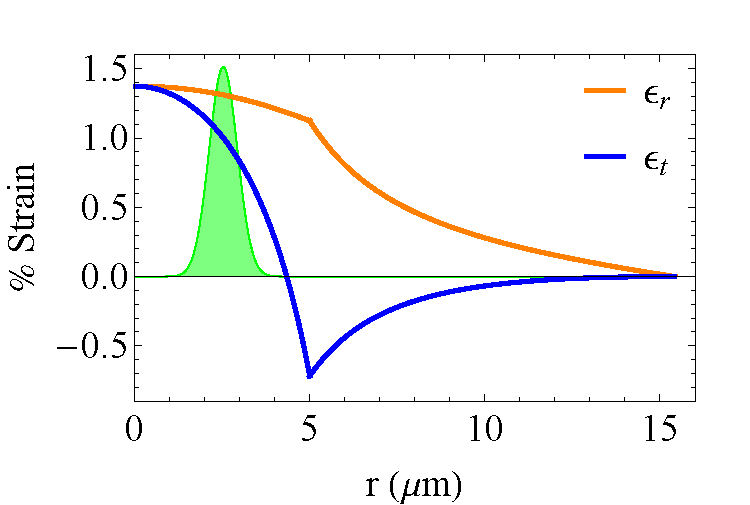
\includegraphics{Figs_Fit/SB02-1_StrainWithLaser.pdf}
	\caption[Laser excitation profile overlaid on strain distribution]{\label{Fig:Fit:FiniteSpot}Laser excitation profile overlaid on the best fit strain distribution for the $\sim 5 \ \mu m$ radius monolayer graphene sealed microchamber with 0.80 MPa of applied pressure.}
	\end{center}
\end{figure}

It should be noted that when the suspended graphene is pushed into the microchamber, it is also pushed slightly out of the focal plane.
This effect is minimal; the confocal length of a 514 nm laser with a 0.81 $\mathrm{\mu}$m beam waste is 4 $\mathrm{\mu}$m, yielding a beam expansion of $<3\%$ for the $<1 \ \mathrm{\mu m}$ graphene deflections encountered in the experiments.
This was considered small enough to ignore.

The finite spot size is accounted for by integrating over the spectra contributed by each point weighted by the excitation point spread function.
Each point contributes a spectra with two Lorentzian peaks centered at
\begin{align*}
	\omega^+ (\rho)&=\omega_0(\rho)-\omega_0(\rho) \gamma(\epsilon_{r}(\rho)+\epsilon_{t}(\rho)) 
		+ \frac{1}{2} \beta (\epsilon_{r}(\rho)-\epsilon_{t}(\rho)) \\
	\omega^-(\rho)&=\omega_0(\rho)-\omega_0(\rho) \gamma(\epsilon_{r}(\rho)+\epsilon_{t}(\rho))
		- \frac{1}{2} \beta (\epsilon_{r}(\rho)-\epsilon_{t}(\rho)) \ .
\end{align*}
The resulting spatial dependence of the Raman spectra is
\begin{equation*}
	g(\rho,\omega)=
	\frac{\left(\frac{1}{2} \Gamma(\rho) \right)^2}
	{\left(\omega-\omega^+(\rho) \right)^2+\left(\frac{1}{2} \Gamma(\rho) \right)^2}+
	\frac{\left(\frac{1}{2} \Gamma(\rho) \right)^2}
	{\left(\omega-\omega^-(\rho) \right)^2+\left(\frac{1}{2} \Gamma(\rho) \right)^2} \ ,
\end{equation*}
A position dependence is given to $\omega_0(\rho)$ and $\Gamma(\rho)$ because the suspended graphene is in general less doped than supported graphene.
This is taken into account by treating $\omega_0(\rho)$ and $\Gamma(\rho)$ as step functions which change value at the edge of the microchamber.

To match the spectra, the excitation point spread function should be expressed as an envelope function along the radial direction with the origin at the center of the microchamber.
Accounting for the point spread function, the shape of the measured spectra is given by
\begin{align*}
	f(\omega,\rho_{\star})&=
		\int \int \mathrm{dx} \ \mathrm{dy} \ e^{-\frac{(x-x_{\star})^2+y^2}{2 \sigma^2}} \ g(\sqrt{x^2+y^2}/R,\omega) \\
	&=e^{-\frac{r_{\star}^2}{2 \sigma^2}} \int  \mathrm{dr} \ r \ e^{-\frac{r^2}{2 \sigma^2}} g(r/R,\omega) 
		\int \mathrm{d \theta} \ e^{\frac{r r_{\star} \mathrm{cos}(\theta)}{\sigma^2}} \\
	&=2\pi R^2 \ e^{-\rho_{\star}^2/2 \bar{\sigma}^2} \int \mathrm{d \rho} \ g(\rho,\omega) \
		\rho \ e^{-\rho^2/2 \bar{\sigma}^2} \
		\mathrm{I}_{0} \left( \frac{\rho \rho_{\star}}{\bar{\sigma}^2} \right) \\
	&\propto \frac{1}{Norm(\rho_{\star})} \int \mathrm{d \rho} \ g(\rho,\omega) \ P(\rho,\rho_{\star}) \ ,
\end{align*}
where $x_{\star}$, $r_{\star}$, and $\rho_{\star}$ are the position of the laser in Cartesian, cylindrical, and normalized cylindrical coordinates respectively, $\sigma$, is equal to half the beam waste, $\bar{\sigma}=\sigma/R$, $\mathrm{I}_0(x)$ is the modified Bessel function of the first kind, and $P(\rho,\rho_{\star})=\rho \ e^{-\rho^2/2 \bar{\sigma}^2} \ \mathrm{I}_0 \left( \frac{\rho \rho_{\star}}{\bar{\sigma}^2} \right)$ is the envelope function.
A normalization constant, $Norm(\rho_{\star})$, which is close to the maximum value of the envelope function was included to keep the widely varying values of the envelope function in a computationally reasonable range.
The maximum of the envelope function is well approximated as
\begin{align*}
	Norm(\rho_{\star})=
		\begin{cases}
			.03 							& , \ \rho_{\star} <    .1 \\
			P(\rho_{\star}, \rho_{\star})	& , \ \rho_{\star} \geq .1 \ ,
		\end{cases}
\end{align*}
and is independent of $\omega$.
Thus, it should be calculated once per spectra as an over head step.

The integral in $f(\omega,\rho_{\star})$ can not be solved analytically.
The strains fields alone are too complex, let alone the additional complexity added by the Lorentzian functions and the envelope function.
Instead, $f(\omega,\rho_{\star})$ must be integrated numerically at each frequency.
Since the form of the strain distribution are different in the domains $[0,1]$, $[1,\rho_0]$, $[\rho_0,\inf]$ it might seem simplest to treat $f(\omega,\rho_{\star})$ as three distinct numeric integrals.
Alternatively, one numerical integral could be used with piecewise functions.
The fastest technique in Wolfram Mathematica 8.0, however, is to minimize the number of numeric integrals without introducing piecewise functions.
The integral over the second domain can be scaled into the first domain using the change of variables $\rho'=\frac{\rho-1}{\rho_0-1}$ giving 
\begin{align*}
	f(\omega,\rho_{\star})=&\int_0^1 \mathrm{d\rho} \left \{ 
	\underbrace{g(\rho,\omega) P(\rho,\rho_{\star})}_{\textrm{inside}} \right. \\ 
	&\left. +\underbrace{(\rho_0-1) g(\rho(\rho_0-1)+1,\omega) P(\rho(\rho_0-1)+1,\rho_{\star})}_{\textrm{outside}}
	\right \} \\
	&+g(\infty,\omega) \underbrace{\int_{\rho_0}^{\infty} \mathrm{d\rho} P(\rho,\rho_{\star})}_{int3(\rho_{\star})} \ .
\end{align*}
Similar to $Norm(\rho_{\star})$, $int3(\rho_{\star})$ is independent of $\omega$ and thus needs to be calculated only once for each $\rho_{\star}$ as an overhead step.
In this way three numeric integrals have been combined into two numeric integrals with one of which only calculated once per $\rho_{\star}$.

Finally, it should be noted that since the numeric integration is the slowest step it should only be calculated once for each $\omega$ in the restrict data domain.
Everything should then reference back to these values.


\section*{Fit linear coefficients}
Having established the predicted shape of the spectra given the current values of the fitting parameters, the modeled spectra needs only to be scaled to match the measured spectra for a comparison to be made.
The scaled modeled spectra is
\begin{equation*}
	model(\omega,\rho_0)=A f(\omega,(\rho_{\star}) + b \ ,
\end{equation*}
where $A$ and $b$ are linear coefficients which correspond to the signal amplitude and the background levels respectively.
These will be independently fit to the measured spectra on a spectra by spectra basis.

Fitting these linear coefficients is much simpler than the non-linear fitting parameters.
Press \emph{et al.} provide a simple matrix method to determine these coefficients \cite{Press2007}.
It is based on the direct minimization of $\chi^2$ by requiring that $\frac{\partial \chi^2}{\partial A}=\frac{\partial \chi^2}{\partial b}=0$.
This yields the system of equations
\begin{equation*}
	\left( \begin{array}{c}
		\sum_j \frac{data_j f(\omega_j,\rho_{\star})}{\sigma_j^2} \\
		\sum_j \frac{data_j                          }{\sigma_j^2}
	\end{array} \right)
	=
	\left( \begin{array}{cc}
		\sum_j \frac{f(\omega_j,\rho_{\star})^2}{\sigma_j^2} & \sum_j \frac{f(\omega_j,\rho_{\star})}{\sigma_j^2} \\
		\sum_j \frac{f(\omega_j,\rho_{\star})}{\sigma_j^2} & \sum_j \frac{1}{\sigma_j^2}
	\end{array} \right)
	\left( \begin{array}{c}
		A \\
		b
	\end{array} \right) \ ,
\end{equation*} 
where $j$ runs over the data points in the restricted domain of the current spectra.
Thus, fitting for the linear coefficients requires only the inversion of a 2 by 2 matrix.

More linear coefficients could be included to account for effects like the different signal intensity for suspended and supported graphene or to allow for different signal intensities from the $G^+$ and $G^-$ peaks.
However, there is no way to restrict the above procedure to give only positive values for the linear coefficients.
Extra coefficients will often lead to non physical, negative coefficients that make the interpretation of the fit metrics more complicated.
Two linear coefficients are enough to capture the complexity of the system while maintaining the simplicity of the fit.

\section*{Add $\chi^2$ to global $\chi^2$}
Having calculated the best possible fit of the hypothetical spectra to the measured data, the goodness of fit can be quantified using the $\chi^2$ metric.
The calculated $\chi^2$ of this spectra should be added to the global $\chi^2$ which includes the $\chi^2$ of each spectra in the data set for the current fitting parameters.
It is also useful to save the linear coefficients so that in the off chance that the current fitting parameters are the best fit, the linear coefficients will not need to be redetermined.

\section*{Select best $\tilde{\chi}^2$ and estimate errors}
After each spectra in the line scan is considered, the global $\chi^2$ is reduced by dividing by the degrees of freedom.
The number of degrees of freedom are equal to the number of fit data points, which was reduced when the fitting domain was restricted, minus the number of fitted parameters, including the 3 fitting parameters and the two linear coefficients per spectra.
This global $\tilde{\chi}^2$ should be saved so that the $\tilde{\chi}^2$ space can be visualized and the minimum found.
It is useful to keep track of the best $\tilde{\chi}^2$ and the corresponding linear coefficients so that the linear coefficients won't need to be refit afterward.

The sampled fitting parameter with the lowest $\tilde{\chi}^2$ best represented the data.
However, these values are not necessarily the best fit.
To ensure that these fitting parameters represent a global minimum and not just a local minimum the $\tilde{\chi}^2$ space should be visualized to.
If only the dimensionless friction was varied, this is done by plotting $\tilde{\chi}^2$ as a function of $F$.
A minimum indicates a best fit.
If all three fitting parameters were varied four dimensional $\tilde{\chi}^2$ space is more difficult to visualize.
One useful way to reduce the dimensionality is to choose the unplotted fitting parameters such that they minimized the $\tilde{\chi}^2$ for the plotted value.
In this way, the plotted values represent the best case scenario.
Figure \ref{fig:Fit:chispace} shows the one dimensional $\tilde{\chi}^2$ space for a fit which included all three fitting parameters.
An obvious minimum in the $\tilde{\chi}^2$ near f=0.14 MPa is visible.

\begin{figure}
	\begin{center}
	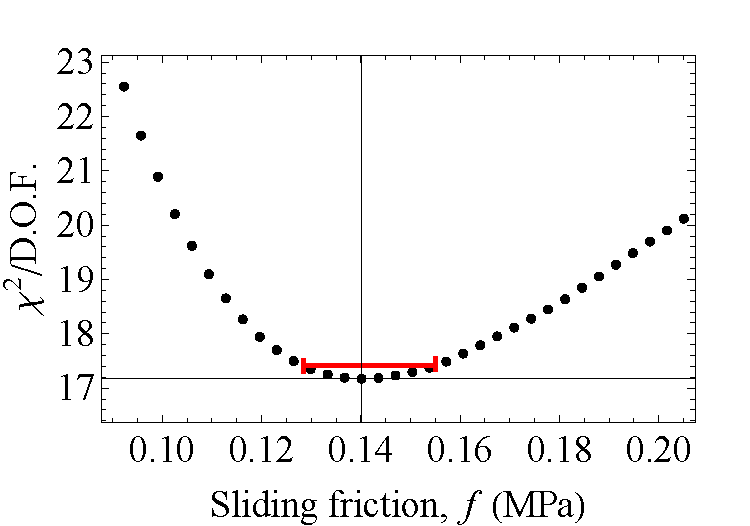
\includegraphics{Figs_Fit/2013-09-05_Fit_101psi_ErrorBar_ForThesis.pdf}
	\end{center}
	\caption[$\tilde{\chi}^2$ as a function of the dimensionless friction]{\label{fig:Fit:chispace}
	$\tilde{\chi}^2$ as a function of the dimensionless friction for the $\sim 5 \ \mu m$ radius monolayer graphene sealed microchamber with 0.80 MPa of applied pressure.
	For each value of $F$, the $\gamma$ and $\beta$ pair which minimized $\tilde{\chi}^2$ was chosen.
	The black cross hair sits at the best fit and the red side ways error bar indicates the uncertainty in the fit based on an increase in $\tilde{\chi}^2$ of 0.25.
	}
\end{figure}

The departure from the minimum of $\tilde{\chi}^2$ can be used to estimate uncertainties in the fitting parameters.
A very steep $\tilde{\chi}^2$ space corresponds to tightly defined fitting parameters.
When viewing the $\tilde{\chi}^2$ space in reduced dimensionality, one needs to be careful that the dimensionality is reduced properly.
Taking a slice in $\tilde{\chi}^2$ space can yield artificially low uncertainties.
Errors in the fitted parameters found by using the increase in $\chi^2$ away from its minimum value \cite{Press2007} are better than one part in one hundred, much smaller than we can claim to have achieved in our experiment.
This discrepancy is due to an underestimation of our uncertainties which include only photon counting and ignore effects due to inhomogeneous doping, sample drift, and laser assisted deposition of dirt on the FLG.
To better illustrate the relative uncertainties amongst different fitted friction values we use a 0.25 increase of $\chi^2$ per degree of freedom above the best fit value to define confidence intervals.
Using this method, the uncertainty in the fitted value in Figure \ref{fig:Fit:chispace} is indicated by the red horizontal error bar.